\documentclass[a4paper,11pt]{article}

%%%%%%%%%%%%%%%%%%%%%%%%%%%%%%%%%%%%%%%%%%%%%%%%%%%%%%%%%%%%%%%%%%%%%%%%
% Paquetes utilizados
%%%%%%%%%%%%%%%%%%%%%%%%%%%%%%%%%%%%%%%%%%%%%%%%%%%%%%%%%%%%%%%%%%%%%%%%

% Gráficos complejos
\usepackage{graphicx}
\usepackage{caption}
\usepackage{subcaption}
\usepackage{placeins}

% Soporte para el lenguaje español
\usepackage{textcomp}
\usepackage[utf8]{inputenc}
\usepackage[T1]{fontenc}
\DeclareUnicodeCharacter{B0}{\textdegree}
\usepackage[spanish]{babel}

% Código fuente embebido
\usepackage{listings}
\usepackage{courier}

% PDFs embebidos para el apéndice
\usepackage{pdfpages}

% Matemáticos
\usepackage{amssymb,amsmath}

% Tablas complejas
\usepackage{multirow}

% Formato de párrafo
\setlength{\parskip}{1ex plus 0.5ex minus 0.2ex}

% Subrayado de palabras
\usepackage[normalem]{ulem}

% Formato de listados de código
\lstset{%
  basicstyle=\footnotesize\ttfamily,
  numberstyle=\tiny,
  numbersep=5pt,
  tabsize=2,
  extendedchars=true,
  breaklines=true,
  stringstyle=\color{white}\ttfamily,
  showspaces=false,
  showtabs=false,
  xleftmargin=17pt,
  framexleftmargin=17pt,
  framexrightmargin=5pt,
  framexbottommargin=4pt,
  showstringspaces=false,
  language=SQL
}
\usepackage{caption}
\DeclareCaptionFont{white}{\color{white}}
\DeclareCaptionFormat{listing}{\colorbox[cmyk]{0.43, 0.35, 0.35,0.01}{\parbox{\textwidth}{\hspace{15pt}#1#2#3}}}
\captionsetup[lstlisting]{format=listing,labelfont=white,textfont=white, singlelinecheck=false, margin=0pt, font={bf,footnotesize}}

%%%%%%%%%%%%%%%%%%%%%%%%%%%%%%%%%%%%%%%%%%%%%%%%%%%%%%%%%%%%%%%%%%%%%%%%
% Título
%%%%%%%%%%%%%%%%%%%%%%%%%%%%%%%%%%%%%%%%%%%%%%%%%%%%%%%%%%%%%%%%%%%%%%%%

% Título principal del documento.
\title{\textbf{Trabajo Práctico: Hiposoft}}

% Información sobre los autores.
\author{%
  Andrés Gastón Arana,     \textit{P. 86.203}                      \\
  Diego Martín Costa,      \textit{P. 78.189}                      \\
  Javier Daniel Zaniratto, \textit{P. 90.886}                      \\
  Sergio Matías Piano,     \textit{P. 85.191}                      \\
  \\
  \normalsize{1er. Cuatrimestre de 2013}                           \\
  \normalsize{75.15 - Bases de datos}                              \\
  \normalsize{Grupo Nro 1}		                           \\
  \normalsize{Docente: Alberto Fasce}	                           \\
  \normalsize{Facultad de Ingeniería, Universidad de Buenos Aires}
}
\date{}

%%%%%%%%%%%%%%%%%%%%%%%%%%%%%%%%%%%%%%%%%%%%%%%%%%%%%%%%%%%%%%%%%%%%%%%%
% Documento
%%%%%%%%%%%%%%%%%%%%%%%%%%%%%%%%%%%%%%%%%%%%%%%%%%%%%%%%%%%%%%%%%%%%%%%%

\begin{document}

% ----------------------------------------------------------------------
% Top matter
% ----------------------------------------------------------------------
\thispagestyle{empty}
\maketitle

\begin{abstract}

  Este informe sumariza el desarrollo del trabajo práctico de la materia Bases
  de Datos (75.15) dictada en el primer cuatrimestre de 2013 en la Facultad de
  Ingeniería de la Universidad de Buenos Aires. El mismo consiste en el
  modelado de datos de un software de administración de eventos hípicos en los
  hipódromos de la provincia de Buenos Aires, cuyos requisitos fueron extraídos
  de un caso de estudio real.

\end{abstract}

\clearpage

% ----------------------------------------------------------------------
% Tabla de contenidos
% ----------------------------------------------------------------------
\tableofcontents
\clearpage


% ----------------------------------------------------------------------
% Desarrollo
% ----------------------------------------------------------------------
\part{Primer entrega}

\section{Metodología y desarrollo}

Primeramente se analizó el enunciado entregado desarrollando un diagrama de
entidad-interrelación inicial plasmando el resultado del análisis.
Posteriormente se refinó el mismo al realizar una investigación de las
características del dominio del problema a resolver; particularmente, se
investigó en publicaciones hípicas de diversa procedencia acerca de las
diferentes relaciones entre jockeys, cuidadores y entrenadores con los studs
que a los que pertenecen los equinos, de manera de poder representar fielmente
en el diagrama las características de dichas relaciones.

Una vez completado y validado el diagrama de entidad interrelación, se
confeccionó el diccionario de datos, cuya elaboración fue trivial considerando
la existencia de dicho diagrama.

Posteriormente, se trabajó en el modelo relacional correspondiente al problema
relevado, mapeando cuidadosamente cada una de las entidades e interrelaciones a
las tablas. Se realizó en este caso también sucesivas aproximaciones al
diagrama final que se presenta en la sección correspondiente de este informe,
analizando las diversas estrategias de mapeo disponibles en cada caso y
seleccionando la más adecuada.

Finalmente, con el modelo relacional completo, se confeccionó un script SQL que
crea las tablas y restricciones correspondientes a dicho modelo utilizando el
subconjunto de instrucciones DDL del lenguaje.

\section{Modelo de entidad-interrelación} \label{sec:der}

\subsection{Hipótesis}

En la confección del diagrama se tomaron como verdaderas las siguientes
hipótesis:

\begin{enumerate}

  \item Los cuidadores y entrenadores trabajan sobre varios equinos al mismo
    tiempo. Cada cuidador y entrenador puede estar trabajando sobre diferentes
    equinos en un momento dado, aunque cada equino posee únicamente un cuidador
    y un entrenador.

  \item Diferentes jockeys pueden correr con diferentes equinos. Cada equino
    participa de una carrera con un jockey particular, pero eso no significa
    que en posteriores carreras deba seguir participando con el mismo jockey.
    Cada jockey puede participar en diferentes carreras con diferentes equinos.

  \item Entrenadores, cuidadores y jockeys trabajan para un stud particular, no
    pudiendo realizar sus tareas correspondientes en equinos de otros studs.

  \item Cada encuentro programado se realiza en su totalidad a lo largo de un
    único día.

\end{enumerate}

Todas estas hipótesis fueron confirmadas consultando a expertos y publicaciones
sobre el dominio del problema. Particularmente, en lo relacionado a la relación
entre los entrenadores, cuidadores y jockeys con los studs, se corroboró que en
el ámbito hípico estos trabajan para una y sólo una caballeriza. Siendo el
enunciado específico en definir stud como tanto el lugar donde reposan los
caballos como la caballeriza, esto indica que entonces el personal está
relacionado con los studs de la forma indicada.

\subsection{Diagrama de entidad-interrelación}

En la figura~\ref{fig:der} se incluye el diagrama de entidad-interrelación
final desarrollado para representar el dominio modelado cuyo relevamiento se
detalla en el enunciado.

\begin{figure}[h!t]
  \centering
  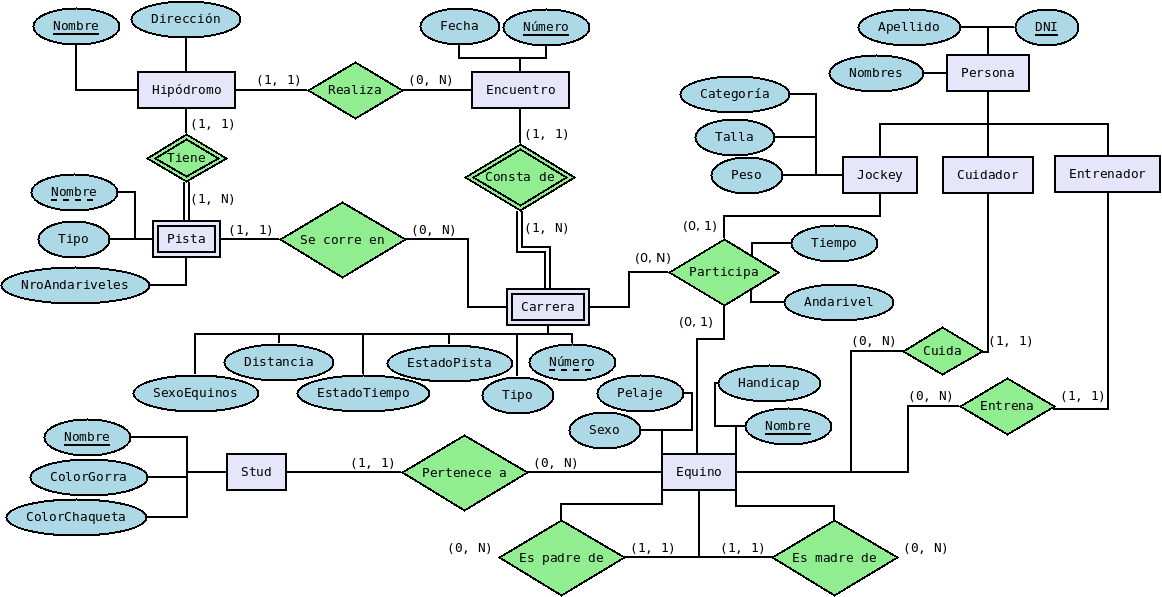
\includegraphics[width=1.5\textwidth, angle=90]{build/images/der.png}
  \caption{Diagrama de entidad-interrelación} \label{fig:der}
\end{figure}

\FloatBarrier

\subsection{Restricciones adicionales}

Las siguientes restricciones adicionales se detallan a continuación por
pertenecer al modelo de entidad-interrelación. No están representadas en el
diagrama dado que su inclusión agregaba complejidad adicional sobre en la
figura que consideramos innecesaria.

\begin{enumerate}

  \item La fecha del encuentro es única entre todos los encuentros.

  \item Cada caballo puede participar únicamente en una carrera por encuentro.
    Los jockeys pueden participar en cuantas carreras se quiera, en cada una de
    ellas con diferentes equinos.

\end{enumerate}

\section{Diccionario de datos}

\subsection{Hipódromo}

Representa una sociedad fundada para contribuir al desarrollo de la crianza de
equinos, que dispone de pistas utilizadas en encuentros programados en los
cuales se disputan las carreras de caballos.

\begin{itemize}

  \item \textbf{\uline{Nombre}} Nombre único descriptivo del hipódromo, como
    puede ser "Hipódromo de San Isidro".

  \item \textbf{Dirección} Dirección completa de la ubicación unívoca en donde
    se encuentran las pistas del hipódromo.

\end{itemize}

\subsection{Realiza}

Representa una relación entre los Hipódromos y los Encuentros, indicando que cada
encuentro se realiza en un Hipódromo. 

\subsection{Encuentro}

Representa un conjunto de carreras equinas que se disputaron o se disputarán de
acuerdo a la planificación anual en un único hipódromo en una fecha
determinada.

\begin{itemize}

  \item \textbf{\uline{Número}} Número correlativo con el que designa al
    encuentro.

  \item \textbf{Fecha} Fecha en la que se desarrollan las carreras del
    encuentro.

  \item \textbf{\dashuline{HipodromoNombre}} Nombre del hipódromo en el que se
    desarrollan las carreras del encuentro.

\end{itemize}

\subsection{Tiene}

Representa una relación entre los Hipódromos y las Pistas, indicando que cada
Hipódromo puede tener 1 o más Pistas. 

\subsection{Pista}

Representa la pista de los hipódromos en donde se realizarán carreras equinas.

\begin{itemize}

  \item \textbf{\uline{Nombre}} Nombre descriptivo de la pista con el que se
    designa la misma.

  \item \textbf{\uline{\dashuline{HipodromoNombre}}} Nombre del hipódromo del
    cual la pista forma parte.

  \item \textbf{Tipo} Indica el materia del piso de la pista, como césped y
    arena.

  \item \textbf{NumeroAndariveles} Cantidad de andariveles disponibles en la
    pista.

\end{itemize}

\subsection{Consta de}

Representa una relación entre los Encuentros y las Carreras, indicando que cada
Encuentro puede estar compuesto por entre 12 y 15 carreras.

\subsection{Carrera}

Representa una competenecia en el que diferentes equinos y jockeys participan
intentando recorrer una distancia dada en una pista en el menor tiempo posible.

\begin{itemize}

  \item \textbf{\uline{Numero}} Número correlativo que identifica la carrera en
    el encuentro.

  \item \textbf{\uline{\dashuline{EncuentroNumero}}} Número del encuentro en el que está
    programada la carrera.

  \item \textbf{Tipo} Clasificación de la carrera de acuerdo a las reglas bajo
    las cuales se determina que equinos y jockeys pueden participar, como ser
    clásicas, handicap, perdedores y de grados.

  \item \textbf{EstadoPista} Indica el estado de la pista al momento de
    disputarse la carrera.

  \item \textbf{EstadoTiempo} Indica las condiciones climatológicas al momento
    de disputarse la carrera.

  \item \textbf{SexoEquinos} Sexo de los equinos que pueden participar en la
    carrera.

  \item \textbf{Distancia} Longitud pactada a recorrer para dar por completada
    la carrera, en metros.

  \item \textbf{Hora} Hora en la que está programada a comenzar la carrera.

  \item \textbf{\dashuline{PistaNombre}} Nombre de la pista en la que se disputa la
    carrera.

  \item \textbf{\dashuline{PistaHipodromoNombre}} Nombre del hipódromo en el cual se
    encuentra la pista en donde se disputa la carrera.

\end{itemize}

\subsection{Se Corre en}

Representa una relación entre las Pistas y las Carreras, indicando que cada
Carrera se corre en 1 Pista.

\subsection{Equino}

Representa a los equinos que podrán participar de las carreras a disputarse en
los encuentros, representando a un stud.

\begin{itemize}

  \item \textbf{\uline{Nombre}} Nombre identificatorio del equino.
    
  \item \textbf{Tipo} Indica la categoría del equino, la cual es utilizada
	para saber en que tipo de carreras puede participar (puede ser perdedor, 
	ganador de primera, de segunda, etc). 
  
  \item \textbf{Pelaje} Indica el color de pelaje que posee el equino (rojo, 
	negro, etc.).
  
  \item \textbf{Sexo} Indica el sexo del equino.
  
  \item \textbf{Handicap} Representa el handicap del equino que permite comparar
	sus ventajas o desventajas respecto a otros equinos.
   
  \item \textbf{\dashuline{StudNombre}} Identificador del stud a cual pertenece el equino.
  
  \item \textbf{\dashuline{PadreNombre}} Identificador del equino padre.
  
  \item \textbf{\dashuline{MadreNombre}} Identificador del equino madre.
  
  \item \textbf{\dashuline{CuidadorPersonaDNI}} Identificador de la persona que se encarga 
	del cuidado del equino (cumpliendo el rol de cuidador).
  
  \item \textbf{\dashuline{EntrenadorPersonaDNI}} Indentificador de la persona encargada 
	del entrenamiento del equino.
  
\end{itemize}

\subsection{Pertenece a}

Representa una relación entre el Equino y el Stud, indicando que cada Equino pertenece a 
1 Stud.

\subsection{Es Padre de}

Representa una relación entre dos Equinos, indicando que un Equino es padre de otro equino.

\subsection{Es Madre de}

Representa una relación entre dos Equinos, indicando que un Equino es madre de otro equino.

\subsection{Entrena}

Representa una relación entre un Equino y un Entrenador, indicando que un equino tiene un
entrenador encargado de Entrenarlo

\subsection{Cuida}

Representa una relación entre un Equino y un Cuidador, indicando que un equino tiene un Cuidador
encargargado de su cuidado.

\subsection{Participación}

Representa la participación de un jockey y un equino en una carrera de un encuentro.
Se utiliza para planificar la participación, y, una vez concluida la carrera,  
guarda el tiempo que le tomó llegar a la meta, el andarivel en el que corrió,
el Peso y la Talla del jockey al momento de la carrera, el Handicap del equino
al momento de la carrera y si fue descalificado o no de la misma. 

\begin{itemize}

  \item \textbf{\uline{\dashuline{JockeyPersonaDNI}}} Identificador de la persona que montó
	al equino (jockey).
  
  \item \textbf{\uline{\dashuline{EquinoNombre}}} Identificador del equino participante.
  
  \item \textbf{\uline{\dashuline{CarreraNúmero}}} Identificador de la carrera.
  
  \item \textbf{\uline{\dashuline{CarreraEncuentroNúmero}}} Identificador del encuentro
        en el cual se había programado la carrera.
  
  \item \textbf{\dashuline{StudNombre}} Identificador del stud al cual pertenece el equino.
  
  \item \textbf{Tiempo} Indica el tiempo que tardó el equino en recorrer la distancia
	pactada para la carrera.
  
  \item \textbf{Andarivel} Indica el andarivel de la pista en el cual
	corrió el equino.
  
  \item \textbf{PesoJockey} Indica el peso del jockey en el momento de la carrera.
  
  \item \textbf{TallaJockey} Indica la talla del jockey cuando ocurrió la carrera.
  
  \item \textbf{HandicapEquino} Handicap del equino al momento de la carrera.
  
  \item \textbf{Descalificado} Indica si el equino fue descalificado o no
	de la carrera
  
\end{itemize}


\subsection{Cuidador}

Representa a las personas encargadas del cuidado de los equinos.

\begin{itemize}

        \item \textbf{\uline{\dashuline{PersonaDNI}}} DNI del cuidador.
	
\end{itemize}

\subsection{Entrenador}

Representa las personas que se encargan de entrenar a los equinos.

\begin{itemize}

        \item \textbf{\uline{\dashuline{PersonaDNI}}} DNI del entrenador.
	
\end{itemize}

\subsection{Persona}

Representa a una persona física.

\begin{itemize}

	\item \textbf{\uline{DNI}} DNI de la persona.
	
	\item \textbf{Nombres} Nombres de la persona.
	
	\item \textbf{Apellidos} Apellidos de la persona.
	
	\item \textbf{StudNombre} Identificador del stud para el cual trabaja la persona.
	
\end{itemize}

\subsection{Trabaja En}

Representa una relación entre una Persona y un Stud, indicando que todas las personas (cuidadores, 
entrenadores, jockeys) trabajan para un Stud.

\subsection{Jockey}

Representa a los encargados de montar los equinos en las distintas carreras 
de los encuentros disputados en los hipódromos, representando a un stud.

\begin{itemize}

        \item \textbf{\uline{\dashuline{PersonaDNI}}} DNI del jockey.
	
	\item \textbf{Categoría} Categoría del Jockey (dependiendo de la cantidad
	de carreras ganadas puede ser aprendiz o profesional).
	
	\item \textbf{Peso} Peso actual del jockey.
	
	\item \textbf{Talla} Talla actual del jockey.

\end{itemize}

\subsection{Stud}

Representa las entidades dueñas de uno o varios equinos que correrán en los distintos
 encuentros, en representación del mismo.

\begin{itemize}

	\item \textbf{\uline{Nombre}} Identificador del stud.
	
	\item \textbf{ColorGorra} Color de la gorra que usarán los jockeys que 
	representen al stud en una carrera.
	
	\item \textbf{ColorChaqueta} Color de la chaqueta que usarán los jockeys 
	que representen al stud en una carrera.
	
\end{itemize}


\section{Resumen del diccionario}

\begin{itemize}

  \item \emph{Hipodromo}(\uline{Nombre}, Direccion)

  \item \emph{Encuentro}(\uline{Numero}, Fecha, \dashuline{HipodromoNombre})

  \item \emph{Pista}(\uline{Nombre}, \uline{\dashuline{HipodromoNombre}}, 
    Tipo, NumeroAndariveles)

  \item \emph{Carrera}(\uline{Numero}, \uline{\dashuline{EncuentroNumero}}, 
    Tipo, EstadoPista, EstadoTiempo, SexoEquinos, Distancia, \dashuline{PistaNombre}, 
    \dashuline{PistaHipodromoNombre}, Hora)

  \item \emph{Stud}(\uline{Nombre}, ColorChaqueta, ColorGorra)

  \item \emph{Persona}(\uline{DNI}, Nombres, Apellidos, \dashuline{StudNombre})

  \item \emph{Cuidador}(\uline{\dashuline{PersonaDNI}})

  \item \emph{Entrenador}(\uline{\dashuline{PersonaDNI}})

  \item \emph{Jockey}(\uline{\dashuline{PersonaDNI}}, Categoria, Peso, Talla)

  \item \emph{Equino}(\uline{Nombre}, Tipo, Pelaje, Sexo, Handicap, 
    \dashuline{StudNombre}, \dashuline{PadreNombre}, \dashuline{MadreNombre}, 
    \dashuline{CuidadorPersonaDNI}, \dashuline{EntrenadorPersonaDNI})

  \item \emph{Participacion}(\uline{\dashuline{JokeyPersonaDNI}}, 
    \uline{\dashuline{EquinoNombre}}, \uline{\dashuline{CarreraNumero}}, 
    \uline{\dashuline{CarreraEncuentroNumero}}, Tiempo, Andarivel, PesoJockey, 
    TallaJockey, HandicapEquino, \dashuline{StudNombre}, Descalificado)


\end{itemize}

\section{Modelo relacional}

\subsection{Diagrama relacional}

En la figura~\ref{fig:relacional} se incluye un diagrama representativo del
modelo relacional desarrollado para el modelo de entidad-interrelación
detallado en la sección~\ref{sec:der}.

\begin{figure}[h!t]
  \centering
  \includegraphics[width=1.65\textwidth, angle=90]{build/images/rel.png}
  \caption{Modelo relacional} \label{fig:relacional}
\end{figure}

\FloatBarrier

\subsection{Scripts de creación}

A continuación se incluyen los scripts de creación de las tablas del modelo
relacional para ser ejecutado en un sistema de bases de datos que interprete
SQL, particularmente las instrucciones DDL de dicho lenguaje. No se incluyen
las instrucciones, normalmente específicas al motor propiamente dicho, de
creación de usuarios, roles, schemas y bases de datos correspondientes.

\lstinputlisting{sql/schema.sql}

\clearpage

\part{Segunda Entrega}

\section{Modelo de entidad-interrelación} \label{sec:der2}

\subsection{Diagrama de entidad-interrelación (de las modificaciones)}

En la figura~\ref{fig:der2} se incluye el diagrama de entidad-interrelación de
las modificaciones realizadas para la segunda entrega. Solo se incluyen
entidades e interrelaciones nuevas o modificadas respecto de la entrega previa.

\subsection{Modificaciones realizadas}

Las modificaciones realizadas para la segunda entrega fueron:

\begin{enumerate}

  \item La entidad JOCKEY no es mas heredera de la entidad PERSONA, por lo tanto
	ahora tendra los atributos Nombres, Apellido y DNI. Además, un Jockey podrá
	estar asociado a mas de un Stud a través de la nueva interrelación CONTRATA.
  Dicha interrelacióñ tendrá los atributos HonorarioFijo y PorcentajePremio. 

  \item La entidad CUIDADOR ahora tiene el atributo Sueldo.

  \item La entidad ENTRENADOR ahora tiene los atributos FechaBaja y Sueldo. 

  \item La entidad PARTICIPACION ahora tiene el atributo Posición.

  \item Hay una nueva entidad ACCIONISTA que ES UNA persona y hereda los atributos
	de PERSONA. Ademas tiene los atributos no comunes ContribucionFija y 
  PorcentajeParticipacion.
  
  \item La entidad EQUINO ahora esta relaciona con la entidad HIPODROMO a traves
    de la nueva interrelación ALOJA EN. 

  \item Hay una nueva entidad débil MOVIMIENTO con los atributos Fecha, Monto,
    Concepto y Número que se relaciona con la entidad STUD a traves de la interrelación
    TIENE. Ademas, se interrelaciona con la entidad EQUINO a través de la interrelación
    GENERADO POR, que indica que el movimiento se le imputa al EQUINO relacionado. 

  \item Hay una nueva entidad APUESTA que esta relacionada con las entidades Equino, 
    Carrera y Jockey. Tiene atributos Monto y Número. 

  \item Hay una nueva entidad PREMIO que esta relacioanda con la entidad
    CARRERA. Tiene como atributos Posición y Monto.

\end{enumerate}

\begin{figure}[h!t]
  \centering
  \includegraphics[width=1.5\textwidth, angle=90]{build/images/der2.png}
  \caption{Diagrama de entidad-interrelación de las modificaciones} \label{fig:der2}
\end{figure}

\FloatBarrier

\section{Adiciones al diccionario de datos}

\subsection{Accionista}

Representa una persona que en sociedad con otras personas (otros accionistas)
conforman un Stud.

\begin{itemize}

  \item \textbf{\uline{\dashuline{PersonaDNI}}} DNI del accionista.

  \item \textbf{ContribucionFija} Contribución mensual que deberá aportar
    un accionista para el mantenimiento de las actividades del Stud. Es calculada
    en base al porcentaje de participacion del accionsita en el Stud.

  \item \textbf{PorcenParticipacion} Es el porcentaje en el cual el accionista 
  participa de los gastos y de los beneficios del Stud. 

\end{itemize}

\subsection{Cuidador}

Representa a las personas encargadas del cuidado de los equinos.

\begin{itemize}

  \item \textbf{\uline{\dashuline{PersonaDNI}}} DNI del cuidador.

  \item \textbf{Sueldo} Sueldo mensual que el Stud le paga al cuidador.
  
\end{itemize}

\subsection{Entrenador}

Representa las personas que se encargan de entrenar a los equinos.

\begin{itemize}

  \item \textbf{\uline{\dashuline{PersonaDNI}}} DNI del entrenador.

  \item \textbf{Sueldo} Sueldo mensual que el Stud le paga al entrenador.

  \item \textbf{FechaBaja} Fecha en la cual el entrenador fue removido del 
    último Stud en el que trabajó. Debe pasar al menos un año para poder
    trabajar en otro Stud. 
  
\end{itemize}

\subsection{Alojado En}

Representa una relacion entre un Equino y el Hipódromo en el cual
se encuentra la caballeriza en la que se aloja el Equino.

\subsection{Jockey}

Representa a los encargados de montar los equinos en las distintas carreras 
de los encuentros disputados en los hipódromos, representando a un stud.

\begin{itemize}

  \item \textbf{\uline{DNI}} DNI del Jockey.
  
  \item \textbf{Nombres} Nombres del Jockey.
  
  \item \textbf{Apellidos} Apellidos del Jockey.

  \item \textbf{Categoría} Categoría del Jockey (dependiendo de la cantidad
  de carreras ganadas puede ser aprendiz o profesional).
  
  \item \textbf{Peso} Peso actual del jockey.
  
  \item \textbf{Talla} Talla actual del jockey.  
  
\end{itemize}

\subsection{Contrata}

Representa la relación entre un Stud, y un Jockey, contratado por el Stud, para
participar en las Carreras de los Encuentros con los Equinos del Stud.

\begin{itemize}

  \item \textbf{\uline{\dashuline{StudNombre}}} Identificador del stud que contrata
    al Jockey.

  \item \textbf{\uline{\dashuline{JockeyDNI}}} Identificador del Jockey que es
    contratado por el stud.

  \item \textbf{HonorarioFijo} Monto que el Jockey percibe del Stud por cada
    participación en una Carrera montando un Equino del Stud.
  
  \item \textbf{PorcentajePremio} Porcentaje que el Jockey percibe de los premios
    recibidos por los Studs por las Carreras ganadas por dicho Jockey.
    
\end{itemize}

\subsection{Apuesta}

Representa una apuesta realizada por un apostador sobre la participación de un Equino
montado por un Jockey en una Carrera. El apostador apuesta una suma de dinero a que
el equino llega en primera posición en dicha carrera.

\begin{itemize}

  \item \textbf{\uline{\dashuline{JockeyDNI}}} Identificador del Jockey que monta
    al equino en la Participación en la que se apuesta.

  \item \textbf{\uline{\dashuline{EquinoNombre}}} Identificador del equino al cual
    se apuesta.
  
  \item \textbf{\uline{\dashuline{CarreraNúmero}}} Identificador de la carrera en la 
    cual se apuesta.
  
  \item \textbf{\uline{\dashuline{CarreraEncuentroNúmero}}} Identificador del encuentro
    al cual pertence la carrera en la que se apuesta

  \item \textbf{\uline{Número}} Identificador de la apuesta.

  \item \textbf{Monto} Suma de dinero que el apostador apostó al caballo en la
    Carrera.

\end{itemize}

\subsection{Tiene}

Representa una relación entre un Stud y un Movimiento Contable.

\subsection{Generado Por}

Representa una relación entre un Equino y un Movimiento. Indica a cual equino puede
imputarsele un determinado movimiento, ya sea gasto, o ganancia. 

\subsection{Movimiento}

Representa un movimiento contable de un Stud. Todos los movimientos de caja
del stud (cobro de premios, pago de canon al Hipódromo, gastos de veterinario, 
comida, etc) son registrados en esta entidad.

\begin{itemize}

  \item \textbf{\uline{\dashuline{StudNombre}}} Identificador del stud a cual pertenece el movimiento

  \item \textbf{\uline{Número}} Indica el número de movimiento.

  \item \textbf{Fecha} Indica la fecha del movimiento.

  \item \textbf{Monto} Indica el monto del movimiento. Si es negativo, es un 
  gasto o salida de dinero. Si es positivo, es un cobro o entrada de dinero.

  \item \textbf{Concepto} Indica el Concepto del Movimiento, por ejemplo 
  'cobro de premio' o 'pago a veterinario'.

  \item \textbf{\dashuline{EquinoNombre}} Identificador del equino al cual se le imputa el movimiento.
      
\end{itemize}

\subsection{Premio}

Representa el monto a ganar como premio, dada una posición, en una carrera.

\begin{itemize}

  \item \textbf{\uline{\dashuline{CarreraNumero}}} Identificador de la carrera
    a la que pertenece este premio.

  \item \textbf{\uline{\dashuline{CarreraEncuentroNumero}}} Identificador del
    encuentro al que pertenece la carrera de este premio.

  \item \textbf{\uline{Posicion}} Indica la posición en la que debe llegar un
    participante para poder reclamar este premio.

  \item \textbf{Monto} Indica el monto con el que se premia la participación.

\end{itemize}

\section{Resumen del Diccionario (de las modificaciones)}

\begin{itemize}

  \item \emph{Accionista}(\uline{\dashuline{PersonaDNI}}, ContribucionFija,
    PorcenParticipacion)

  \item \emph{Cuidador}(\uline{\dashuline{PersonaDNI}}, Sueldo)

  \item \emph{Entrenador}(\uline{\dashuline{PersonaDNI}}, Sueldo, FechaBaja)

  \item \emph{Jockey}(\uline{DNI}, Categoria, Peso, Talla, Nombres, Apellido)

  \item \emph{Movimiento}(\uline{\dashuline{StudNombre}}, \uline{Numero},
    Fecha, Monto, Concepto, \dashuline{EquinoNombre})

  \item \emph{Apuesta}(\uline{\dashuline{JockeyDNI}},
    \uline{\dashuline{EquinoNombre}}, \uline{\dashuline{CarreraNumero}},
    \uline{\dashuline{CarreraEncuentroNumero}}, \uline{Numero}, Monto)

  \item \emph{Contrata}(\uline{\dashuline{StudNombre}},
    \uline{\dashuline{JockeyDNI}}, HonorarioFijo, PorcentajePremio)

  \item \emph{Premio}(\uline{\dashuline{CarreraNumero}},
    \uline{\dashuline{CarreraEncuentroNumero}}, \uline{Posición}, Monto)

\end{itemize}

\section{Modelo Relacional completo}

\subsection{Diagrama relacional}

En la figura~\ref{fig:rel2} se incluye un diagrama representativo del
modelo relacional completo desarrollado para el modelo de entidad-interrelación
modificado para la segunda entrega.

\begin{figure}[h!t]
  \centering
  \includegraphics[width=1.5\textwidth, angle=90]{build/images/rel2.png}
  \caption{Modelo relacional} \label{fig:rel2}
\end{figure}

\FloatBarrier

\subsection{Scripts de Modificación}

A continuación se incluyen los scripts de modificación de las tablas
existentes, y creación de las tablas nuevas, para crear la estructura de la
base de datos necesaria para soportar el modelo detallado en las secciones
anteriores.

\lstinputlisting{sql/schema2.sql}

\clearpage

\section{Consultas}

A continuación se enumeran las consultas pedidas en el trabajo práctico y las
soluciones a cada una de ellas, de acuerdo al modelo de datos desarrollado.

\subsection{Consulta 1}

Se pide el monto total ganado por el jockey Juan Arias en el año 2011 por
comisión de apuestas.

\begin{lstlisting}

  SELECT 
    SUM(premio.monto * contratacion.porcentaje_premio)
  FROM
    participacion,
    carrera,
    encuentro,
    jockey,
    premio,
    stud,
    contratacion,
  WHERE
    participacion.carrera_numero = carrera.numero
    AND participacion.carrera_encuentro_numero = carrera.encuentro_numero
    AND encuentro.numero = carrera.encuentro_numero
    AND jockey.dni = participacion.jockey_dni
    AND premio.carrera_numero = carrera.numero
    AND premio.carrera_encuentro_numero = carrera.encuentro_numero
    AND stud.nombre = participacion.stud_nombre
    AND contratacion.jockey_dni = jockey.dni
    AND contratacion.stud_nombre = stud.nombre
    AND jockey.nombres = Juan Arias
    AND encuentro.fecha >= 01/01/2011
    AND encuentro.fecha <= 31/12/2011

\end{lstlisting}

\subsection{Consulta 2}

Se pide el Stud que gasto más recursos para obtener cada premio.

\begin{lstlisting}
  SELECT 
    stud 
  FROM
    promedio_gasto_por_premio pgpp
  WHERE 
    NOT EXISTS(SELECT * 
               FROM 
                 promedio_gasto_por_premio pgpp2
               WHERE 
                 pgpp2.promedio_gasto > pgpp.promedio_gasto AND 
                 pgpp2.stud = pgpp.stud)
\end{lstlisting}

\subsection{Consulta 3}

Se pide encontrar los caballos que mejores resultados económicos generaron para
sus Studs.

\begin{lstlisting}
 
  SELECT 
    stud, 
    equino 
  FROM
    balance_por_stud_equino bpse
  WHERE
    NOT EXISTS (SELECT * 
                FROM 
                  balance_por_stud_equino bpse2
                WHERE 
                  bpse.resultado < bpse2.resultado AND 
                  bpse.stud = bpse2.stud)

\end{lstlisting}

\part{Apéndice}
\appendix

\section{Enunciado original}\label{sec:enunciado}

\includepdf[pages={-}, frame=true, pagecommand={}, noautoscale=true, scale=0.7]{docs/enunciado.pdf}

\section{Enunciado segunda entrega}\label{sec:enunciado}
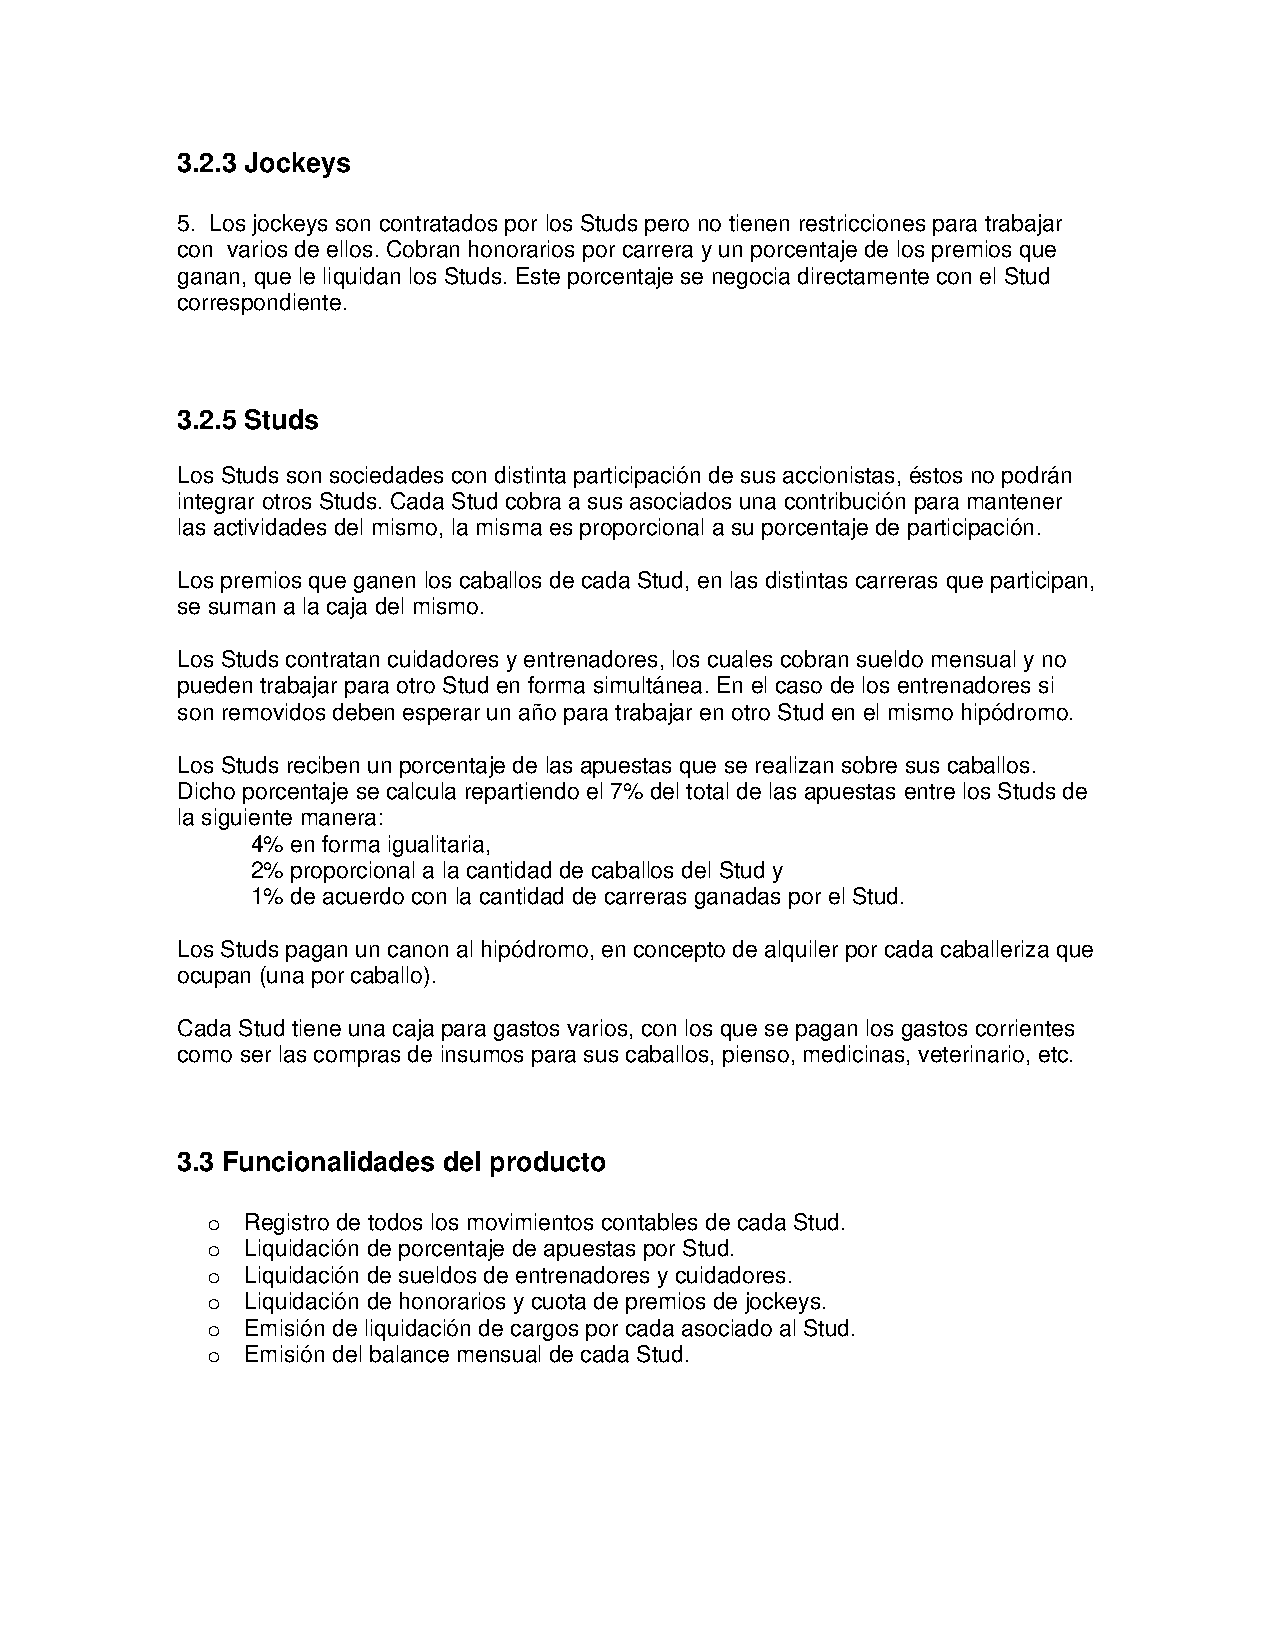
\includepdf[pages={-}, frame=true, pagecommand={}, noautoscale=true, scale=0.7]{docs/TP0106.pdf}


\end{document}

